%inicio Daniel
\chapter{Skiplists}

\chaplabel{skiplists}

In this chapter, we discuss a beautiful data structure: the skiplist,
which has a variety of applications.  Using a skiplist we can implement a
#List# that has $O(\log n)$ time implementations of #get(i)#, #set(i,x)#,
#add(i,x)#, and #remove(i)#. We can also implement an #SSet# in which
all operations run in $O(\log #n#)$ expected time.
%Finally, a skiplist can be used to implement a #Rope# in which all
%operations run in $O(\log #n#)$ time.

The efficiency of skiplists relies on their use of randomization.
When a new element is added to a skiplist, the skiplist uses random coin
tosses to determine the height of the new element.  The performance of
skiplists is expressed in terms of expected running times and path
lengths. This expectation is taken over the random coin tosses used by
the skiplist.  In the implementation, the random coin tosses used by a
skiplist are simulated using a pseudo-random number (or bit) generator.

\section{The Basic Structure}

\index{skiplist}%
Conceptually, a skiplist is a sequence of singly-linked lists
$L_0,\ldots,L_h$. Each list $L_r$ contains a subset of the items
in $L_{r-1}$.  We start with the input list $L_0$ that contains #n#
items and construct $L_1$ from $L_0$, $L_2$ from $L_1$, and so on.
The items in $L_r$ are obtained by tossing a coin for each element, #x#,
in $L_{r-1}$ and including #x# in $L_r$ if the coin turns up as heads.
This process ends when we create a list $L_r$ that is empty.  An example
of a skiplist is shown in \figref{skiplist}.

\begin{figure}
  \begin{center}
    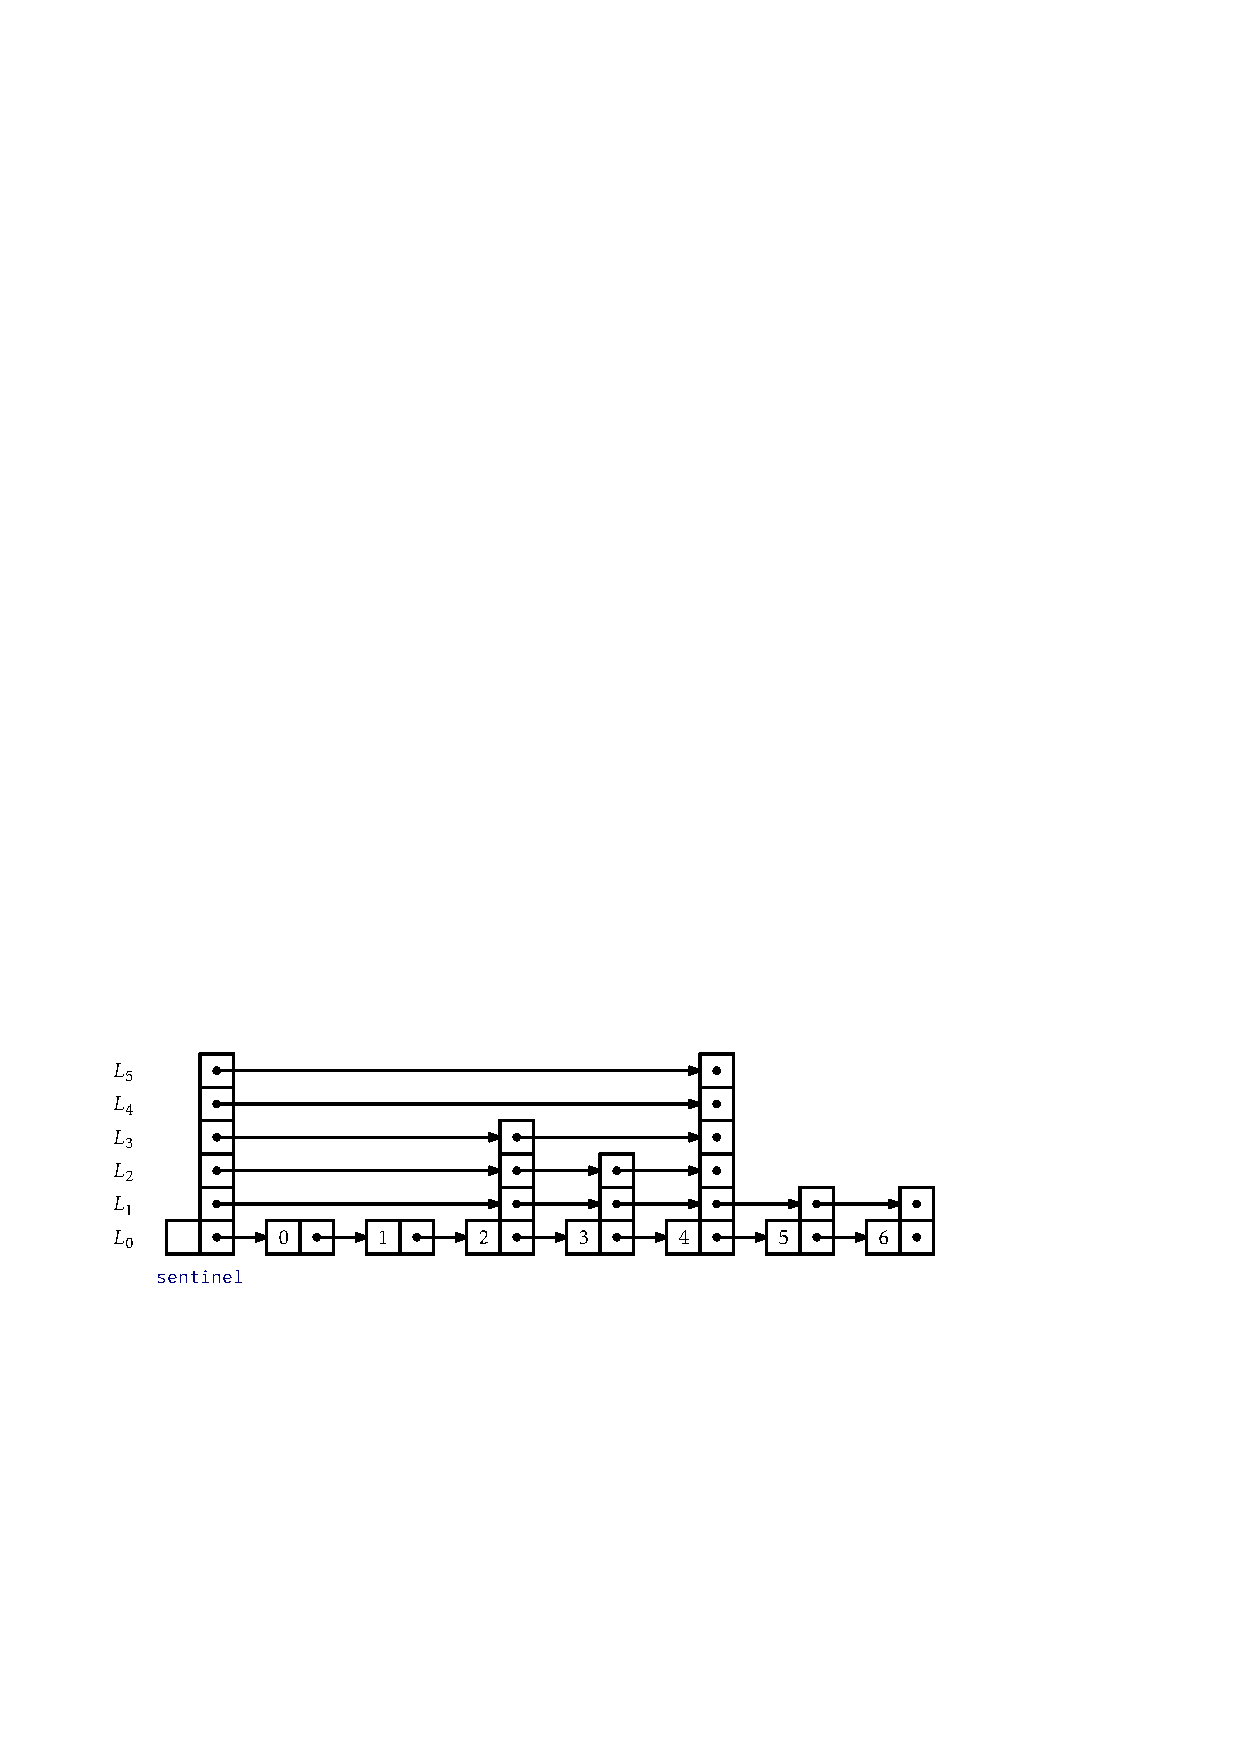
\includegraphics[width=\ScaleIfNeeded]{figs/skiplist}
  \end{center}
  \caption{A skiplist containing seven elements.}
  \figlabel{skiplist}
\end{figure}

For an element, #x#, in a skiplist, we call the \emph{height}
\index{height!of a skiplist}%
of #x# the
largest value $r$ such that #x# appears in $L_r$.  Thus, for example,
elements that only appear in $L_0$ have height $0$.  If we spend a few
moments thinking about it, we notice that the height of #x# corresponds
to the following experiment:  Toss a coin repeatedly until it comes
up as tails.  How many times did it come up as heads?  The answer, not
surprisingly, is that the expected height of a node is 1. (We expect to
toss the coin twice before getting tails, but we don't count the last
toss.) The \emph{height} of a skiplist is the height of its tallest node.

At the head of every list is a special node, called the \emph{sentinel},
\index{sentinel node}%
that acts as a dummy node for the list. The key property of skiplists
is that there is a short path, called the \emph{search path}, 
\index{search path!in a skiplist}%
from the
sentinel in $L_h$ to every node in $L_0$.  Remembering how to construct
a search path for a node, #u#, is easy (see \figref{skiplist-searchpath})
:  Start at the top left corner of your skiplist (the sentinel in $L_h$)
and always go right unless that would overshoot #u#, in which case you
should take a step down into the list below.

More precisely, to construct the search path for the node #u# in $L_0$,
we start at the sentinel, #w#, in $L_h$.  Next, we examine #w.next#.
If #w.next# contains an item that appears before #u# in $L_0$, then
we set $#w#=#w.next#$.  Otherwise, we move down and continue the search
at the occurrence of #w# in the list $L_{h-1}$.  We continue this way
until we reach the predecessor of #u# in $L_0$. 
\begin{figure}
  \begin{center}
    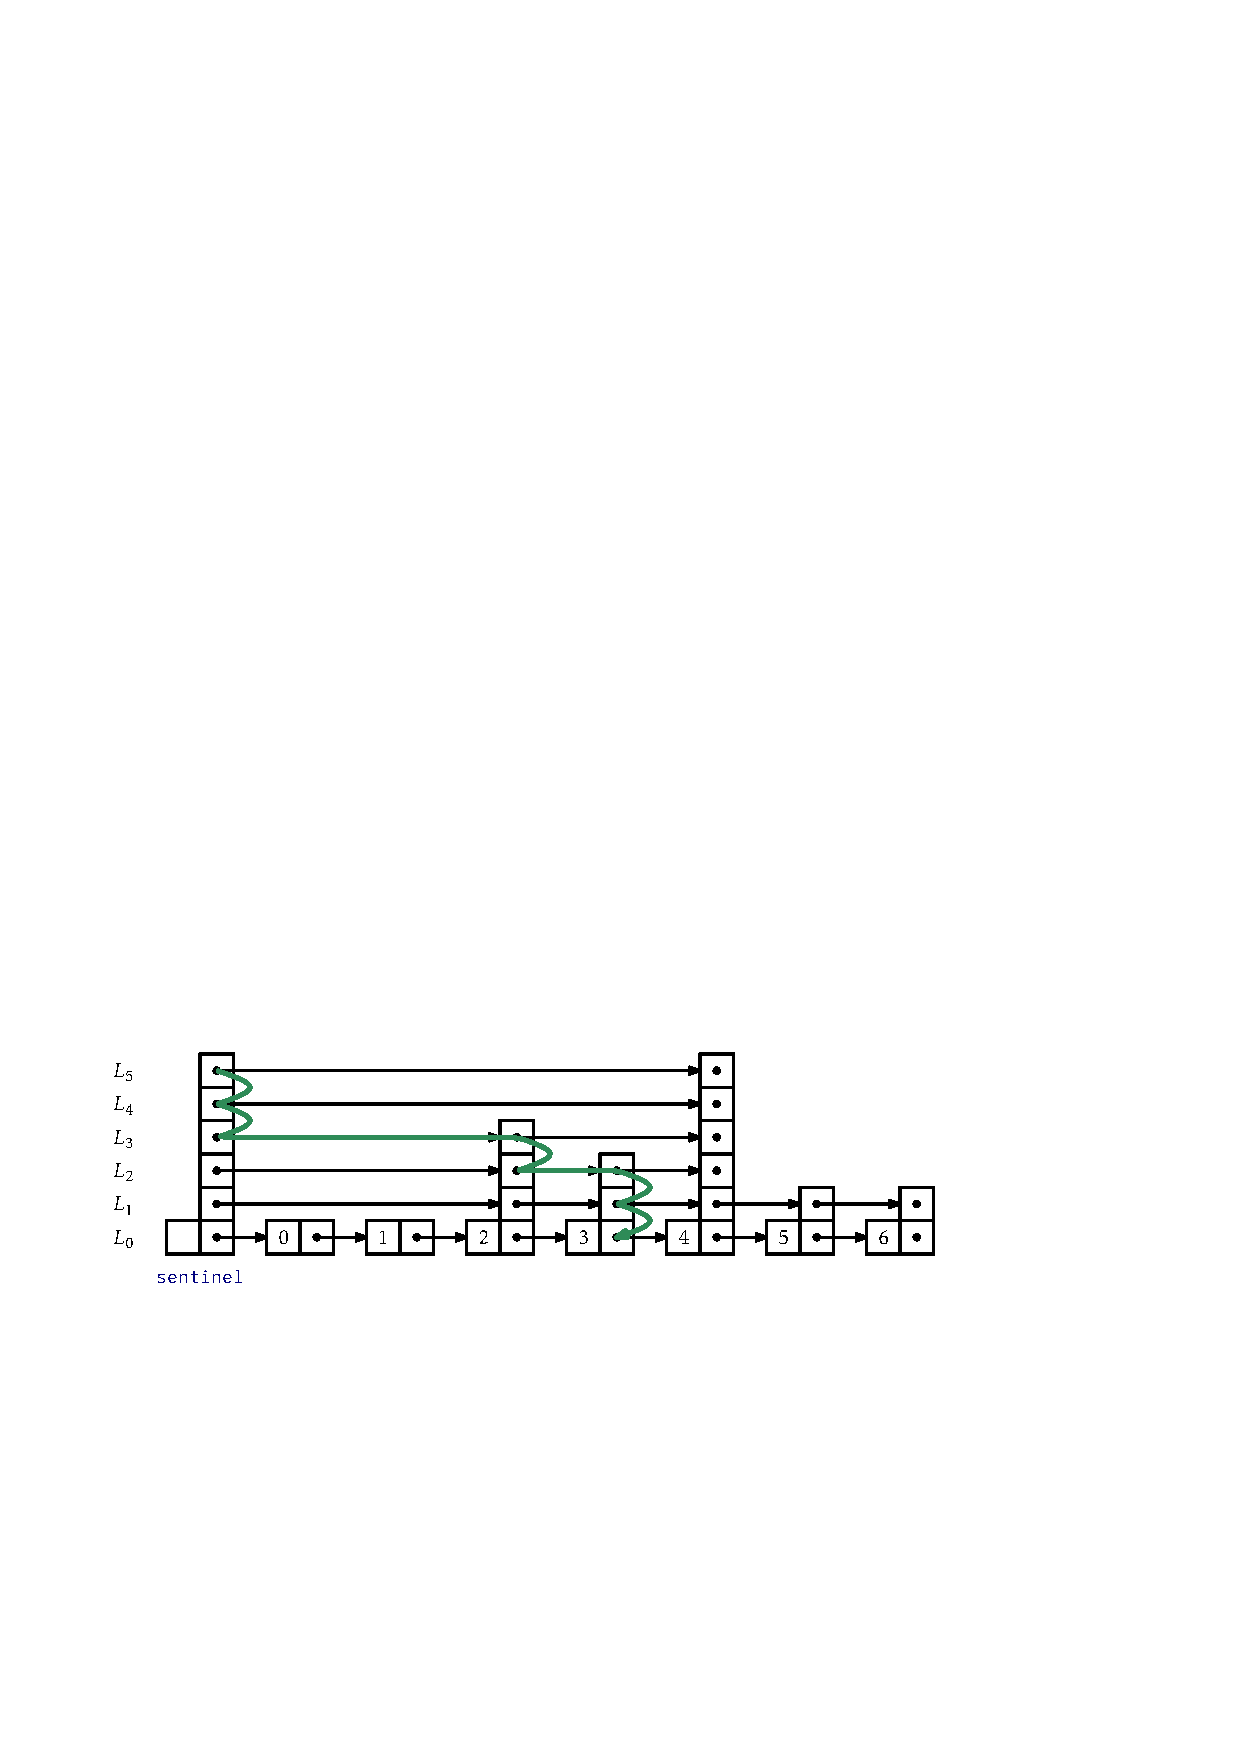
\includegraphics[width=\ScaleIfNeeded]{figs/skiplist-searchpath}
  \end{center}
  \caption{The search path for the node containing $4$ in a skiplist.}
  \figlabel{skiplist-searchpath}
\end{figure}
%Fim Daniel

%inicio Diana
The following result, which we will prove in \secref{skiplist-analysis},
shows that the search path is quite short:

\begin{lem}\lemlabel{skiplist-searchpath}
The expected length of the search path for any node, #u#, in $L_0$ is at
most $2\log #n# + O(1) = O(\log #n#)$.
\end{lem}

A space-efficient way to implement a skiplist is to define a #Node#,
#u#, as consisting of a data value, #x#, and an array, #next#, of
pointers, where #u.next[i]# points to #u#'s successor in the list
$L_{#i#}$.  In this way, the data, #x#, in a node is
\javaonly{referenced}\cpponly{stored}\pcodeonly{referenced} 
only once, even though #x# may appear in several lists.

\javaimport{ods/SkiplistSSet.Node<T>}
\cppimport{ods/SkiplistSSet.Node}

The next two sections of this chapter discuss two different applications
of skiplists.  In each of these applications, $L_0$ stores the main
structure (a list of elements or a sorted set of elements).
The primary difference between these structures is in how
a search path is navigated; in particular, they differ in how
they decide if a search path should go down into $L_{r-1}$ or go right
within $L_r$.

\section{#SkiplistSSet#: An Efficient #SSet#}
\seclabel{skiplistset}

\index{SkiplistSSet@#SkiplistSSet#}%
A #SkiplistSSet# uses a skiplist structure to implement the #SSet#
interface.   When used in this way, the list $L_0$ stores the elements of
the #SSet# in sorted order.  The #find(x)# method works by following
the search path for the smallest value #y# such that $#y#\ge#x#$:

\codeimport{ods/SkiplistSSet.find(x).findPredNode(x)}

Following the search path for #y# is easy:  when situated at
some node, #u#, in  $L_{#r#}$, we look right to #u.next[r].x#.
If $#x#>#u.next[r].x#$, then we take a step to the right in
$L_{#r#}$; otherwise, we move down into $L_{#r#-1}$.  Each step
(right or down) in this search takes only constant time; thus, by
\lemref{skiplist-searchpath}, the expected running time of #find(x)#
is $O(\log #n#)$.

Before we can add an element to a #SkipListSSet#, we need a method to
simulate tossing coins to determine the height, #k#, of a new node.
We do so by picking a random integer, #z#, and counting the number of
trailing $1$s in the binary representation of #z#:\footnote{This method
does not exactly replicate the coin-tossing experiment since the value of
#k# will always be less than the number of bits in an #int#.  However,
this will have negligible impact unless the number of elements in the
structure is much greater than $2^{32}=4294967296$.}

\codeimport{ods/SkiplistSSet.pickHeight()}

To implement the #add(x)# method in a #SkiplistSSet# we search for #x#
and then splice #x# into a few lists $L_0$,\ldots,$L_{#k#}$, where #k#
is selected using the #pickHeight()# method. The easiest way to do this
is to use an array, #stack#, that keeps track of the nodes at which
the search path goes down from some list $L_{#r#}$ into $L_{#r#-1}$.
More precisely, #stack[r]# is the node in $L_{#r#}$ where the search path
proceeded down into $L_{#r#-1}$.  The nodes that we modify to insert #x#
are precisely the nodes $#stack[0]#,\ldots,#stack[k]#$.  The following
code implements this algorithm for #add(x)#:
\label{pg:skiplist-add}
\codeimport{ods/SkiplistSSet.add(x)}

\begin{figure}
  \begin{center}
    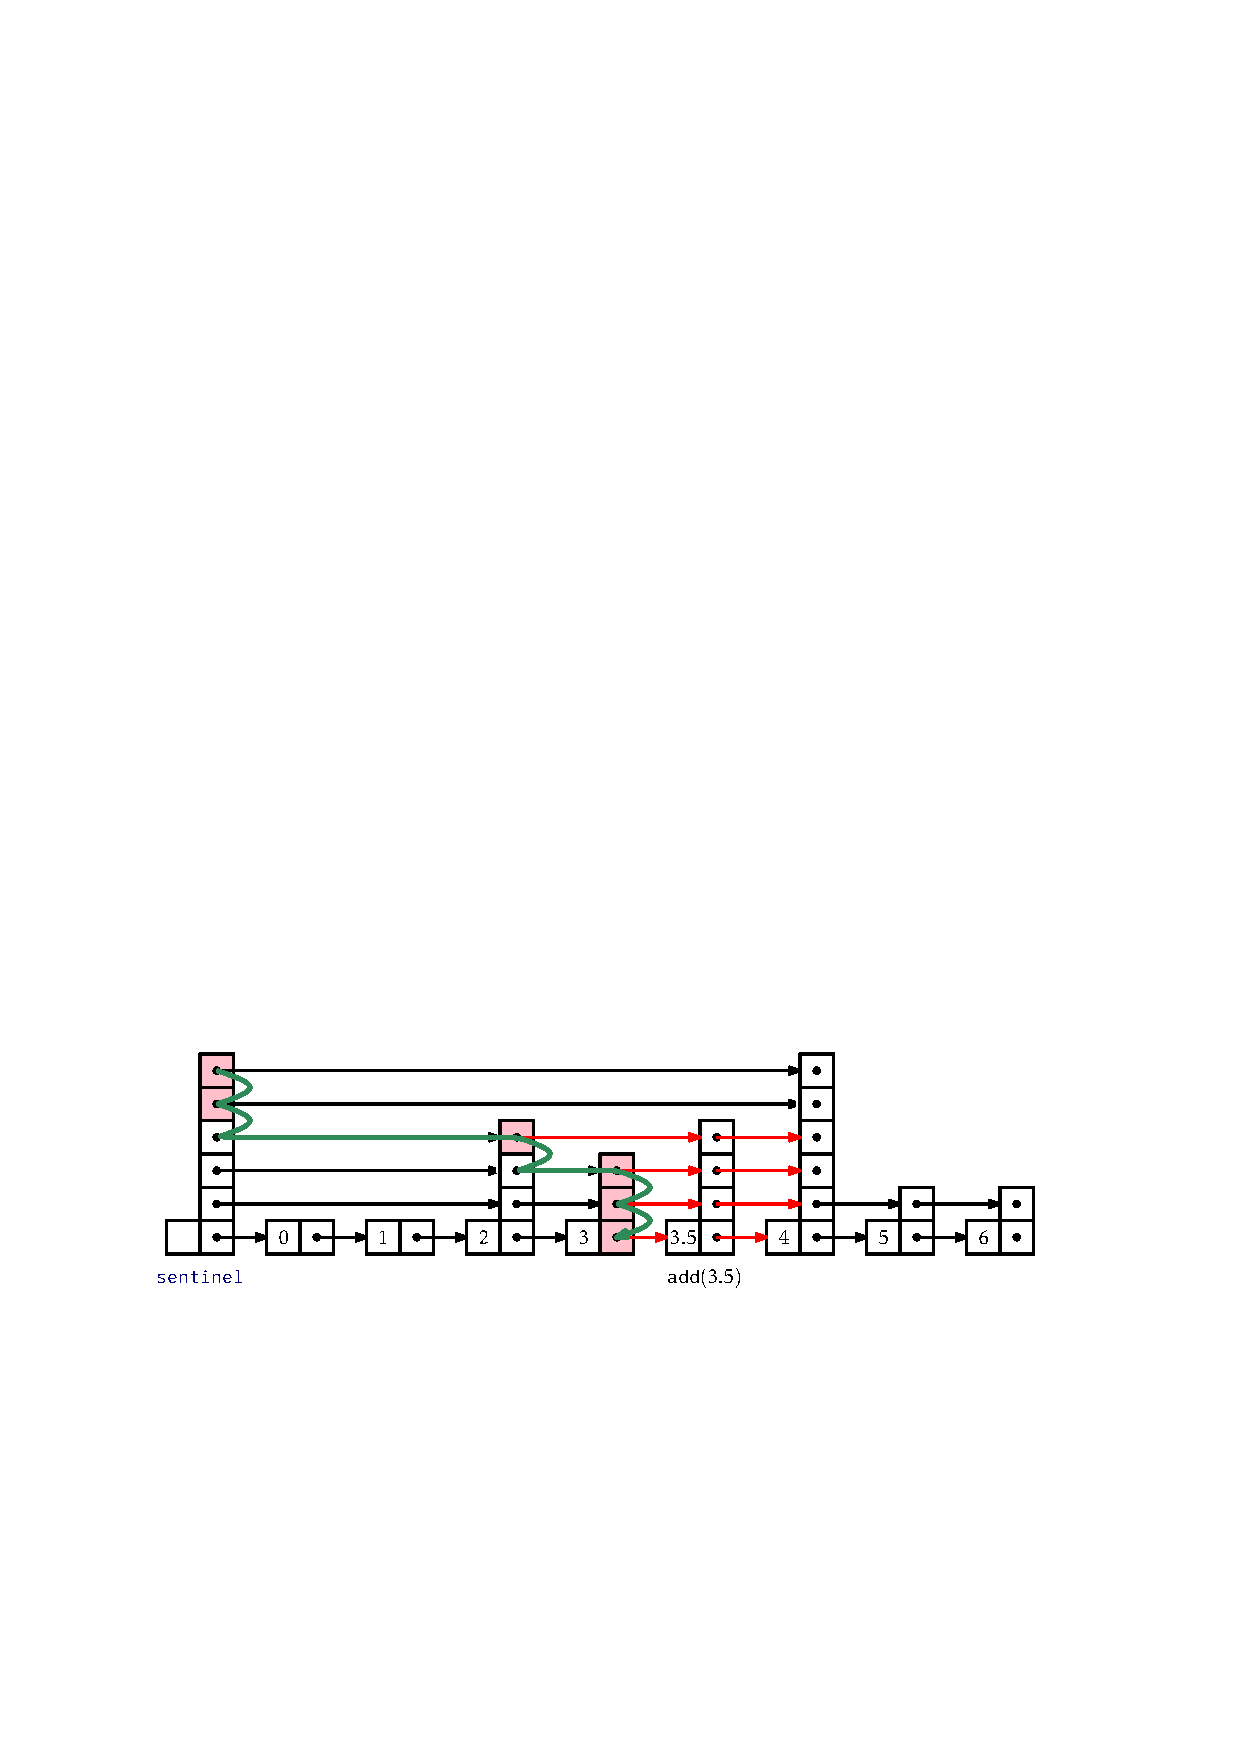
\includegraphics[width=\ScaleIfNeeded]{figs/skiplist-add}
  \end{center}
  \caption[Adding to a skiplist]{Adding the node containing $3.5$ to a skiplist.  The nodes stored in #stack#
  are highlighted.}
  \figlabel{skiplist-add}
\end{figure}
%fim Diana

%inicio Ester
Removing an element, #x#, is done in a similar way, except that there
is no need for #stack# to keep track of the search path.  The removal
can be done as we are following the search path.  We search for #x#
and each time the search moves downward from a node #u#, we check if
$#u.next.x#=#x#$ and if so, we splice #u# out of the list:
\codeimport{ods/SkiplistSSet.remove(x)}

\begin{figure}
  \begin{center}
    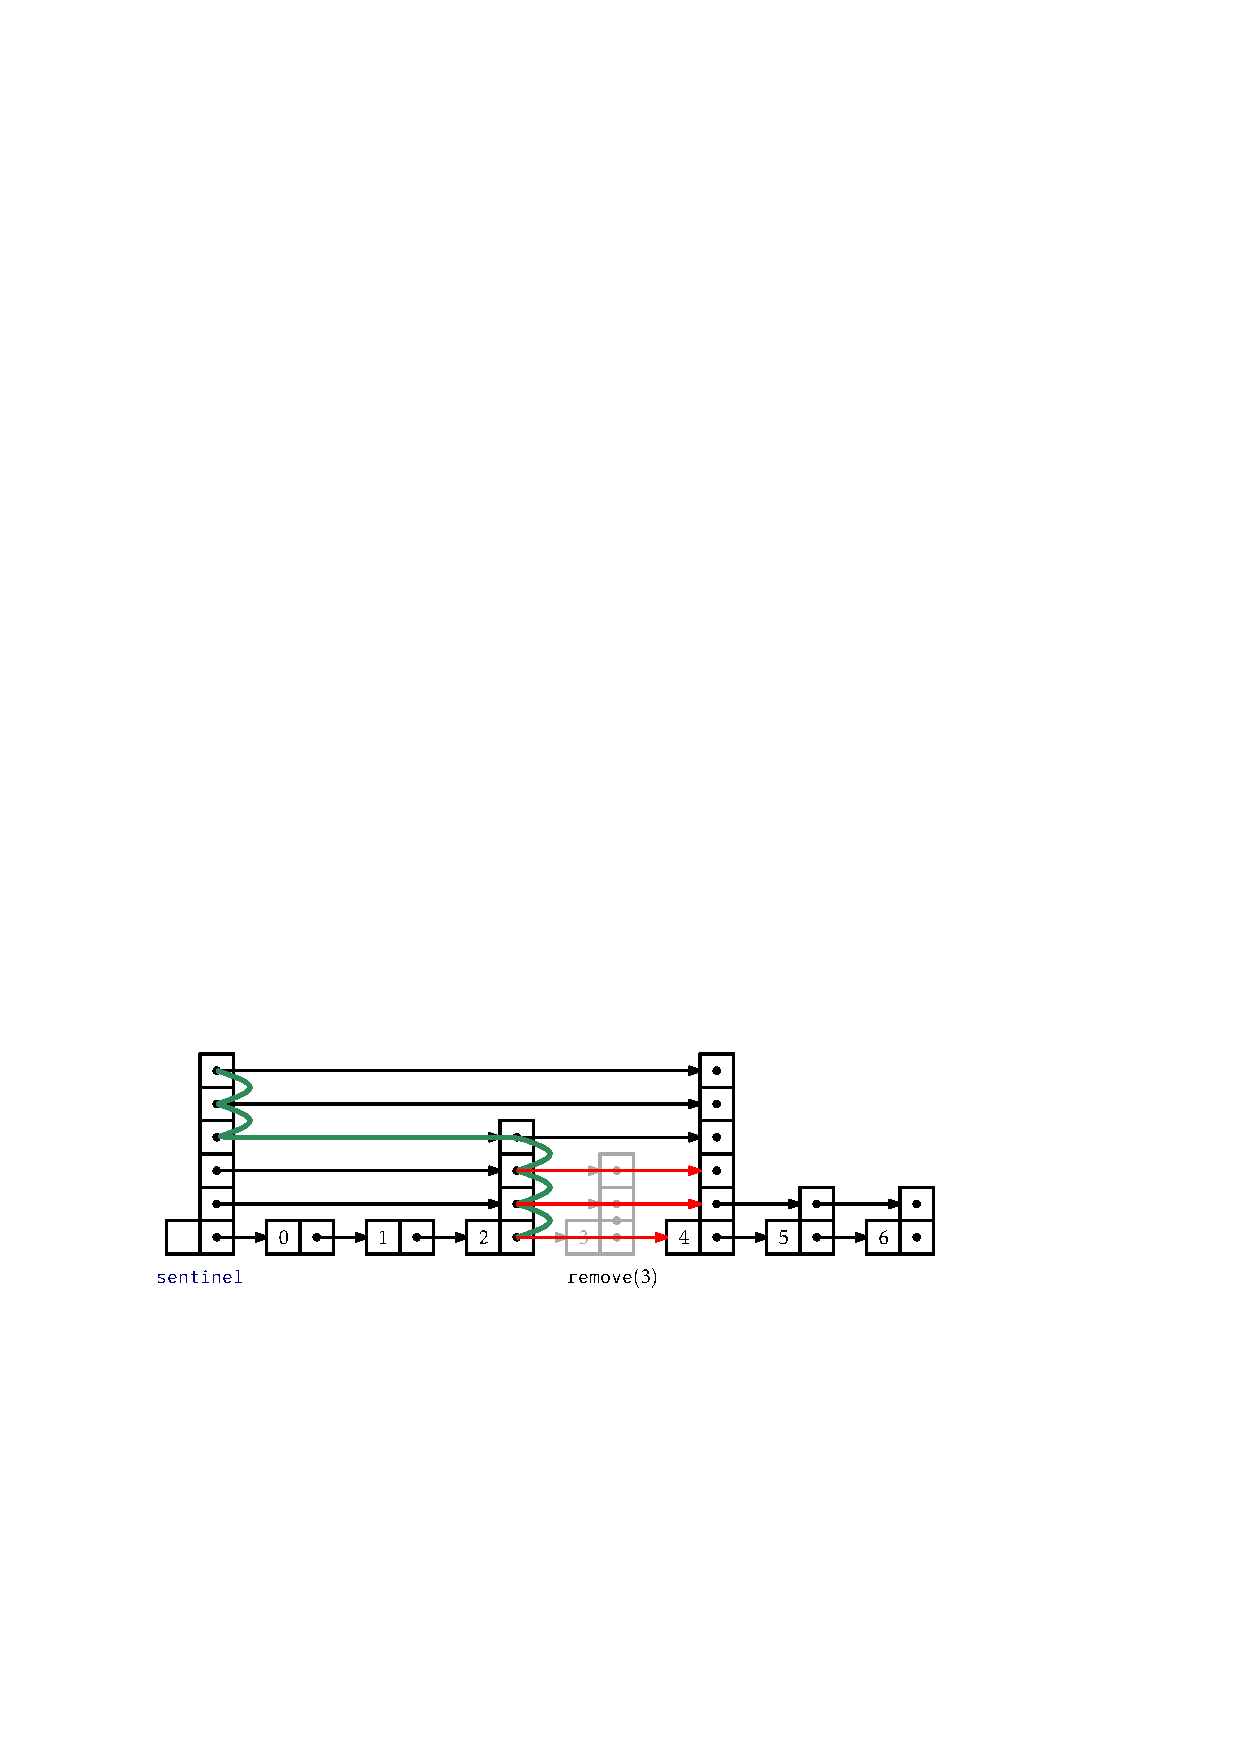
\includegraphics[width=\ScaleIfNeeded]{figs/skiplist-remove}
  \end{center}
  \caption{Removing the node containing $3$ from a skiplist.}
  \figlabel{skiplist-remove}
\end{figure}

\subsection{Summary}

The following theorem summarizes the performance of skiplists when used to
implement sorted sets:

\begin{thm}\thmlabel{skiplist}
#SkiplistSSet# implements the #SSet# interface. A #SkiplistSSet# supports
the operations #add(x)#, #remove(x)#, and #find(x)# in $O(\log #n#)$
expected time per operation.
\end{thm}

\section{#SkiplistList#: An Efficient Random-Access #List#}
\seclabel{skiplistlist}

\index{SkiplistList@#SkiplistList#}%
A #SkiplistList# implements the #List# interface using a skiplist
structure.  In a #SkiplistList#, $L_0$ contains the elements of the
list in the order in which they appear in the list.   As in a
#SkiplistSSet#, elements can be added, removed, and accessed in $O(\log
#n#)$ time.

For this to be possible, we need a way to follow the search path for
the #i#th element in $L_0$.  The easiest way to do this is to define
the notion of the \emph{length} of an edge in some list, $L_{#r#}$.
We define the length of every edge in $L_{0}$ as 1.  The length of an edge, #e#,
in $L_{#r#}$, $#r#>0$, is defined as the sum of the lengths of the edges below #e#
in $L_{#r#-1}$.  Equivalently, the length of #e# is
the number of edges in $L_0$ below #e#.  See \figref{skiplist-lengths} for
an example of a skiplist with the lengths of its edges shown.  Since the
edges of skiplists are stored in arrays, the lengths can be stored the same
way:

\begin{figure}
  \begin{center}
    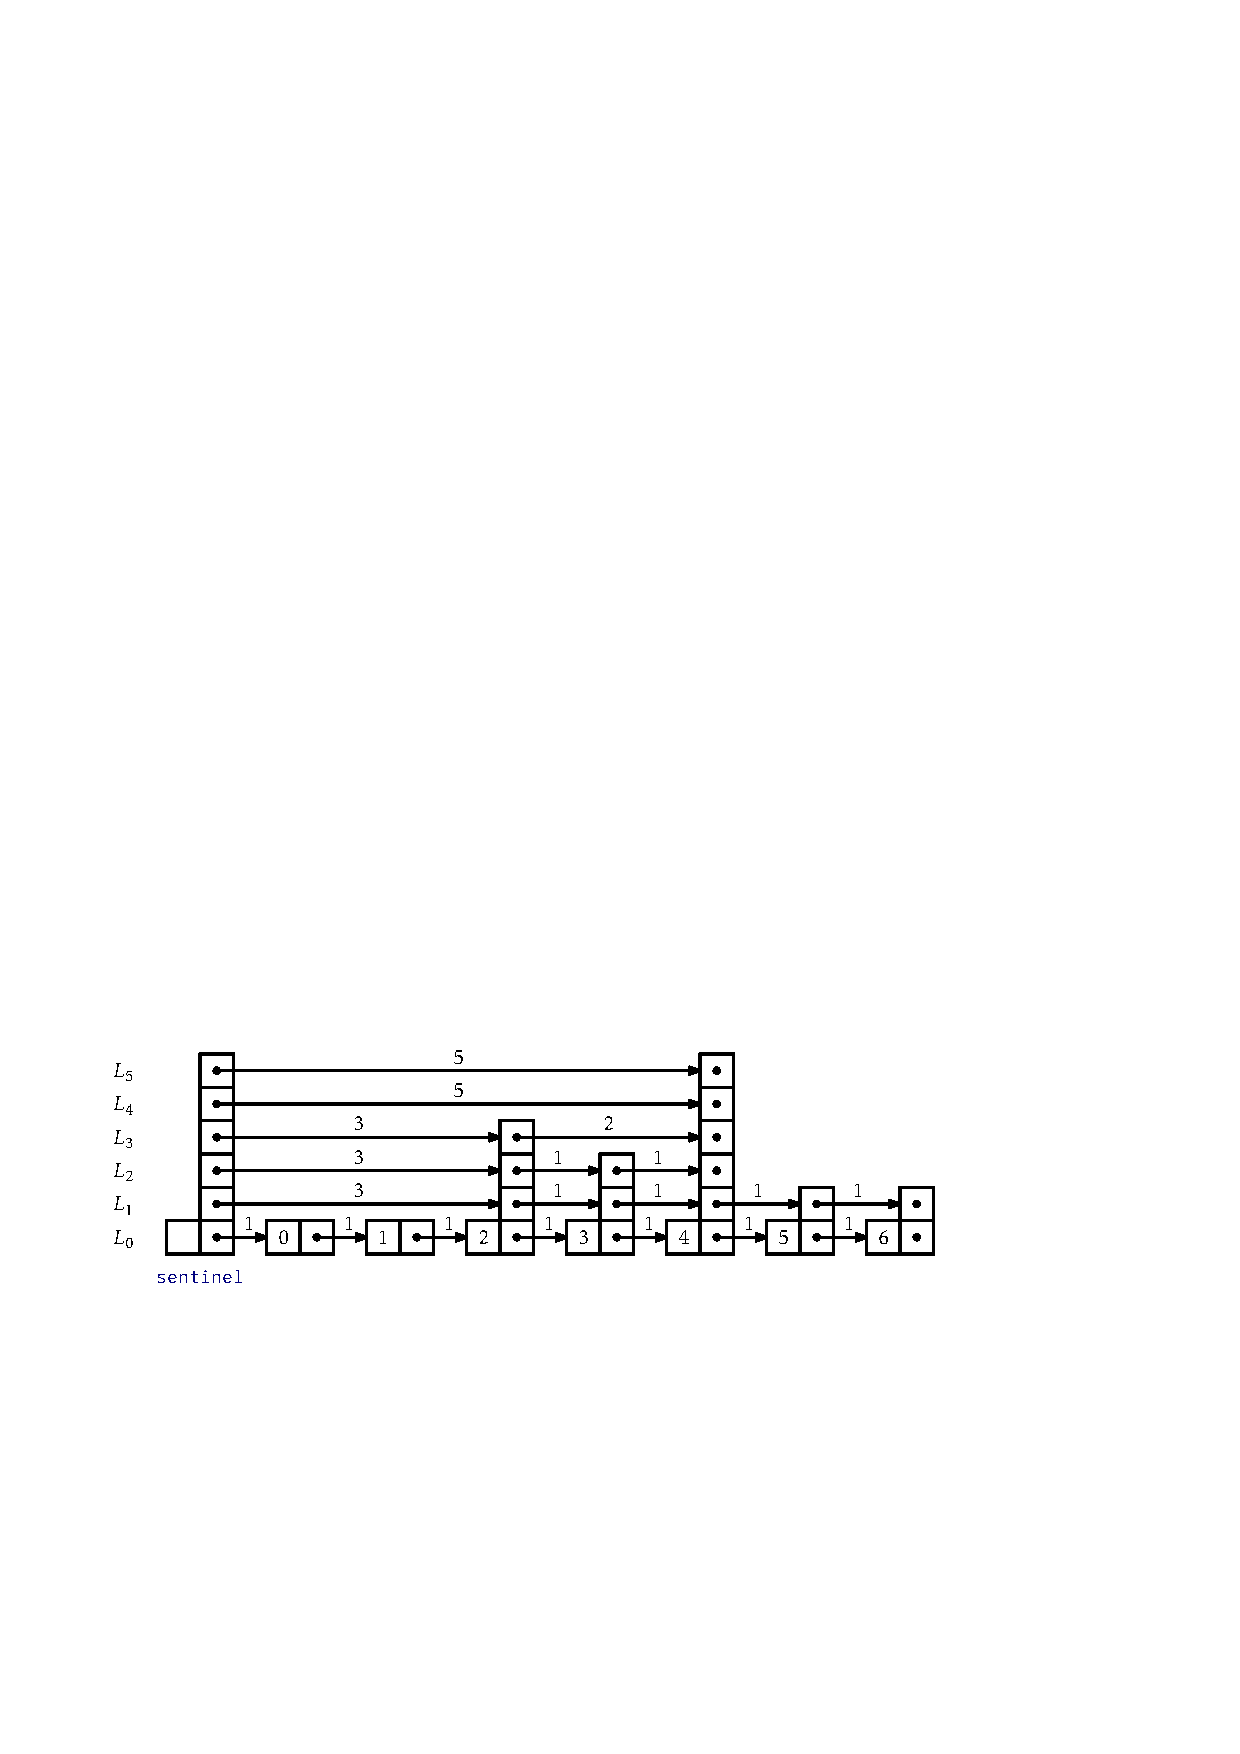
\includegraphics[width=\ScaleIfNeeded]{figs/skiplist-lengths}
  \end{center}
  \caption{The lengths of the edges in a skiplist.}
  \figlabel{skiplist-lengths}
\end{figure}

\javaimport{ods/SkiplistList.Node}
\cppimport{ods/SkiplistList.Node}

The useful property of this definition of length is that, if we are
currently at a node that is at position #j# in $L_0$ and we follow an
edge of length $\ell$, then we move to a node whose position, in $L_0$,
is $#j#+\ell$.  In this way, while following a search path, we can keep
track of the position, #j#, of the current node in $L_0$.  When at a
node, #u#, in $L_{#r#}$, we go right if #j# plus the length of the edge
#u.next[r]# is less than #i#. Otherwise, we go down into $L_{#r#-1}$.

\codeimport{ods/SkiplistList.findPred(i)}
\codeimport{ods/SkiplistList.get(i).set(i,x)}

Since the hardest part of the operations #get(i)# and #set(i,x)# is
finding the #i#th node in $L_0$, these operations run in
$O(\log #n#)$ time.
%fim Ester

%inicio Gabriel
Adding an element to a #SkiplistList# at a position, #i#, is fairly
simple.  Unlike in a #SkiplistSSet#, we are sure that a new
node will actually be added, so we can do the addition at the same time
as we search for the new node's location. We first pick the height, #k#,
of the newly inserted node, #w#, and then follow the search path for #i#.
Any time the search path moves down from $L_{#r#}$ with $#r#\le #k#$, we
splice #w# into $L_{#r#}$.  The only extra care needed is to ensure that
the lengths of edges are updated properly.  See \figref{skiplist-addix}.

\begin{figure}
  \begin{center}
    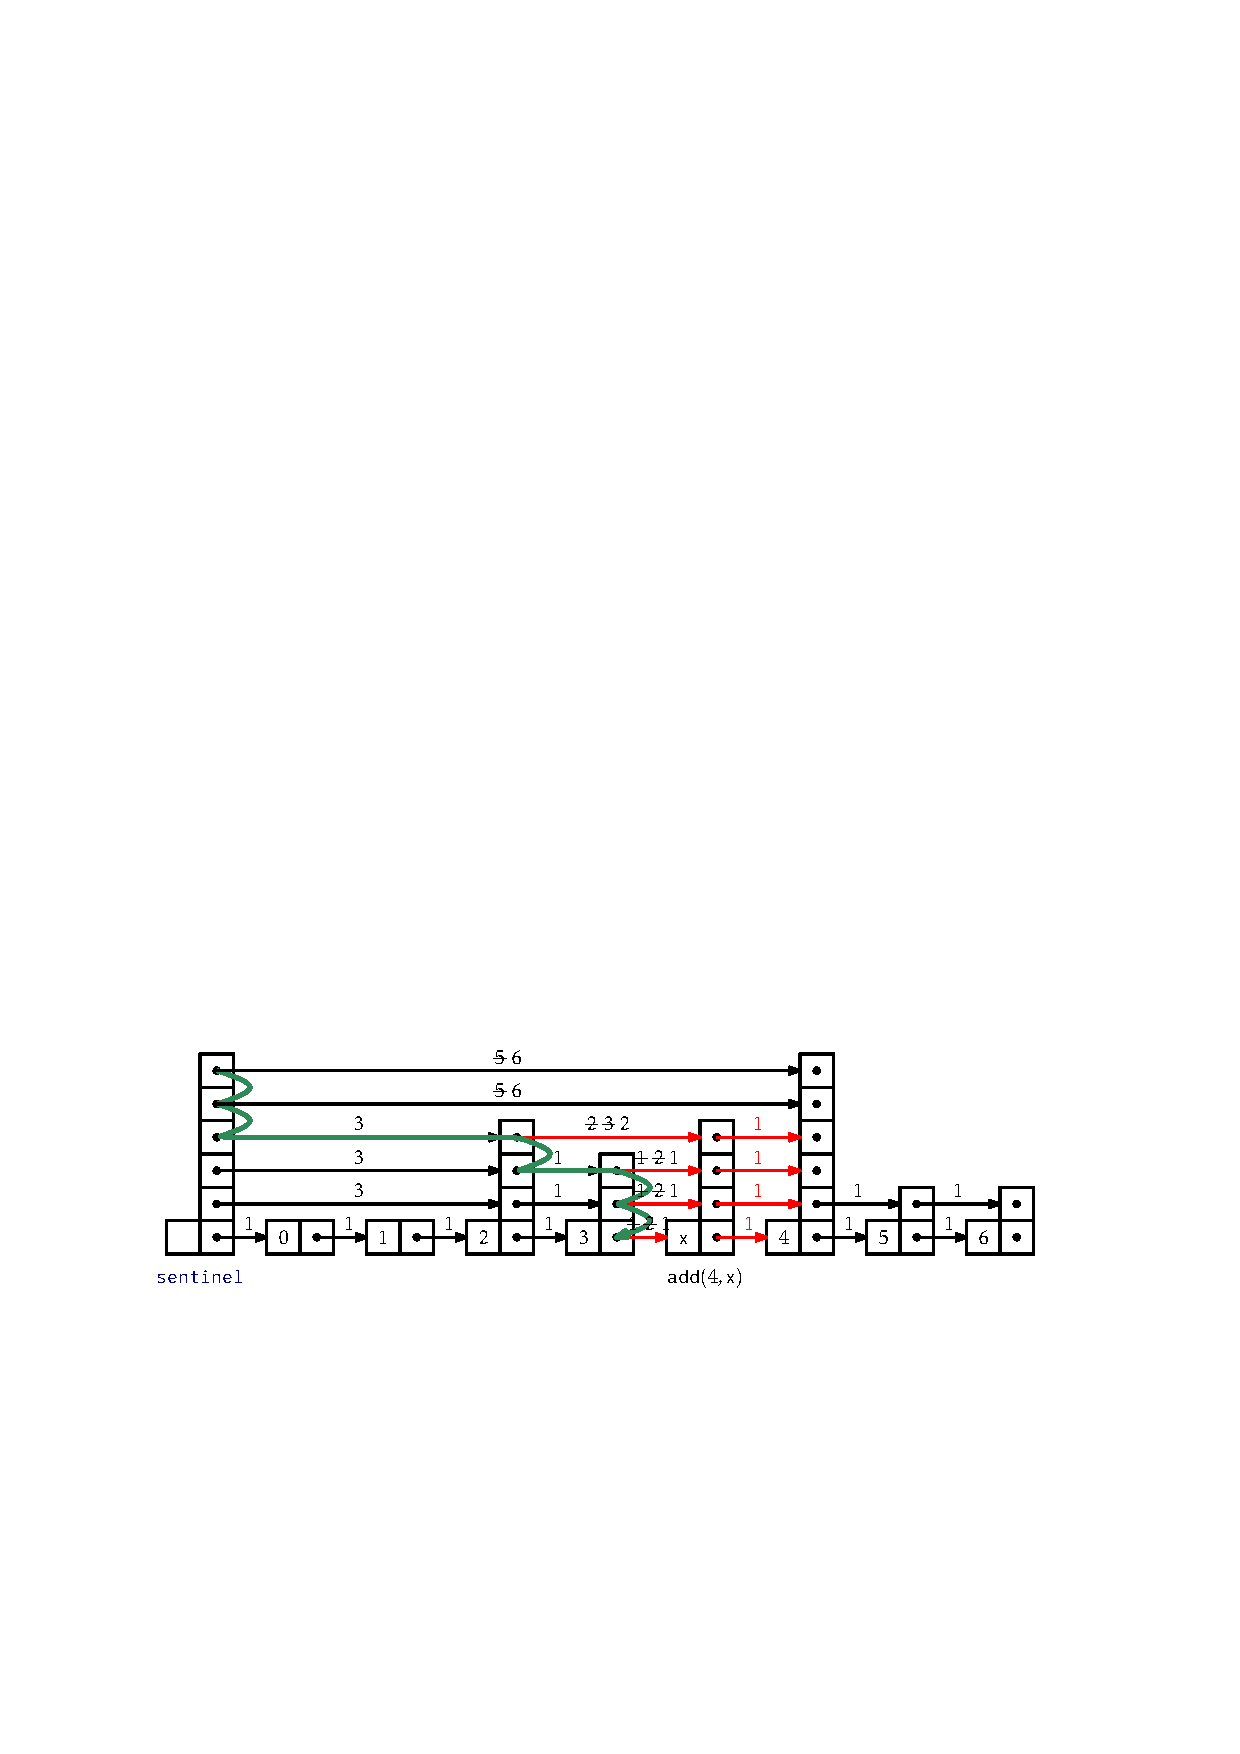
\includegraphics[width=\ScaleIfNeeded]{figs/skiplist-addix}
  \end{center}
  \caption[Adding to a SkiplistList]{Adding an element to a #SkiplistList#.}
  \figlabel{skiplist-addix}
\end{figure}

Note that, each time the search path goes down at a node, #u#, in $L_{#r#}$,
the length of the edge #u.next[r]# increases by one, since we are adding
an element below that edge at position #i#.  Splicing  the node #w# between two nodes,
#u# and #z#, works as shown in \figref{skiplist-lengths-splice}.  While
following the search path we are already keeping track of the position,
#j#, of #u# in $L_0$.  Therefore, we know that the length of the edge from
#u# to #w# is $#i#-#j#$.  We can also deduce the length of the edge
from #w#  to #z# from the length, $\ell$, of the edge from #u# to #z#.
Therefore, we can splice in #w# and update the lengths of the edges in
constant time.

\begin{figure}
  \begin{center}
    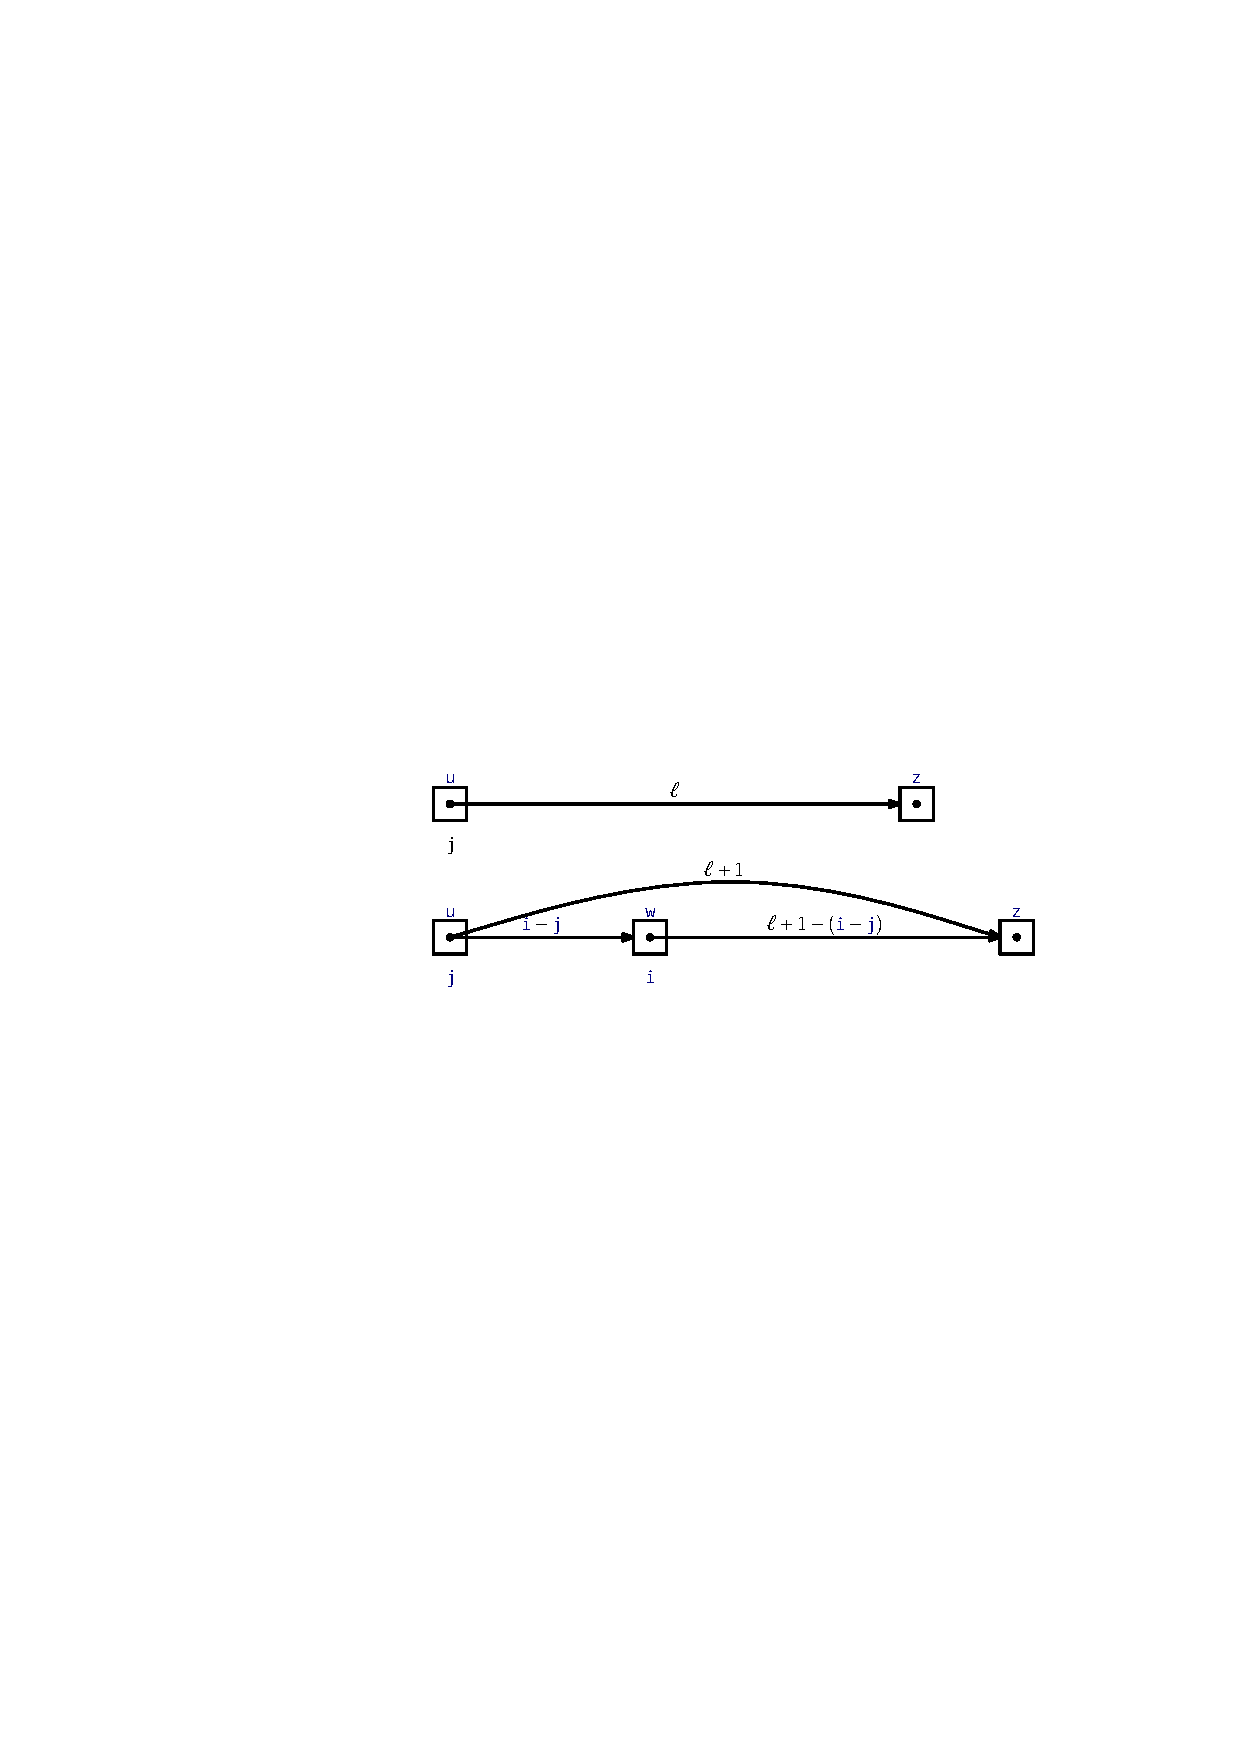
\includegraphics[scale=0.90909]{figs/skiplist-lengths-splice}
  \end{center}
  \caption[Adding to a SkiplistList]{Updating the lengths of edges while splicing a node 
   #w# into a skiplist.}
  \figlabel{skiplist-lengths-splice}
\end{figure}

This sounds more complicated than it is, for the code is actually
quite simple:

\codeimport{ods/SkiplistList.add(i,x)}
\codeimport{ods/SkiplistList.add(i,w)}


By now, the implementation of 
the #remove(i)# operation in a #SkiplistList# should be obvious.  We follow the search path for the node at position #i#.  Each time the search path takes a step down from a node, #u#, at level #r# we decrement the length of the edge leaving #u# at that level.  We also check if #u.next[r]# is the element of rank #i# and, if so, splice it out of the list at that level.   An example is shown in \figref{skiplist-removei}.
\begin{figure}
  \begin{center}
    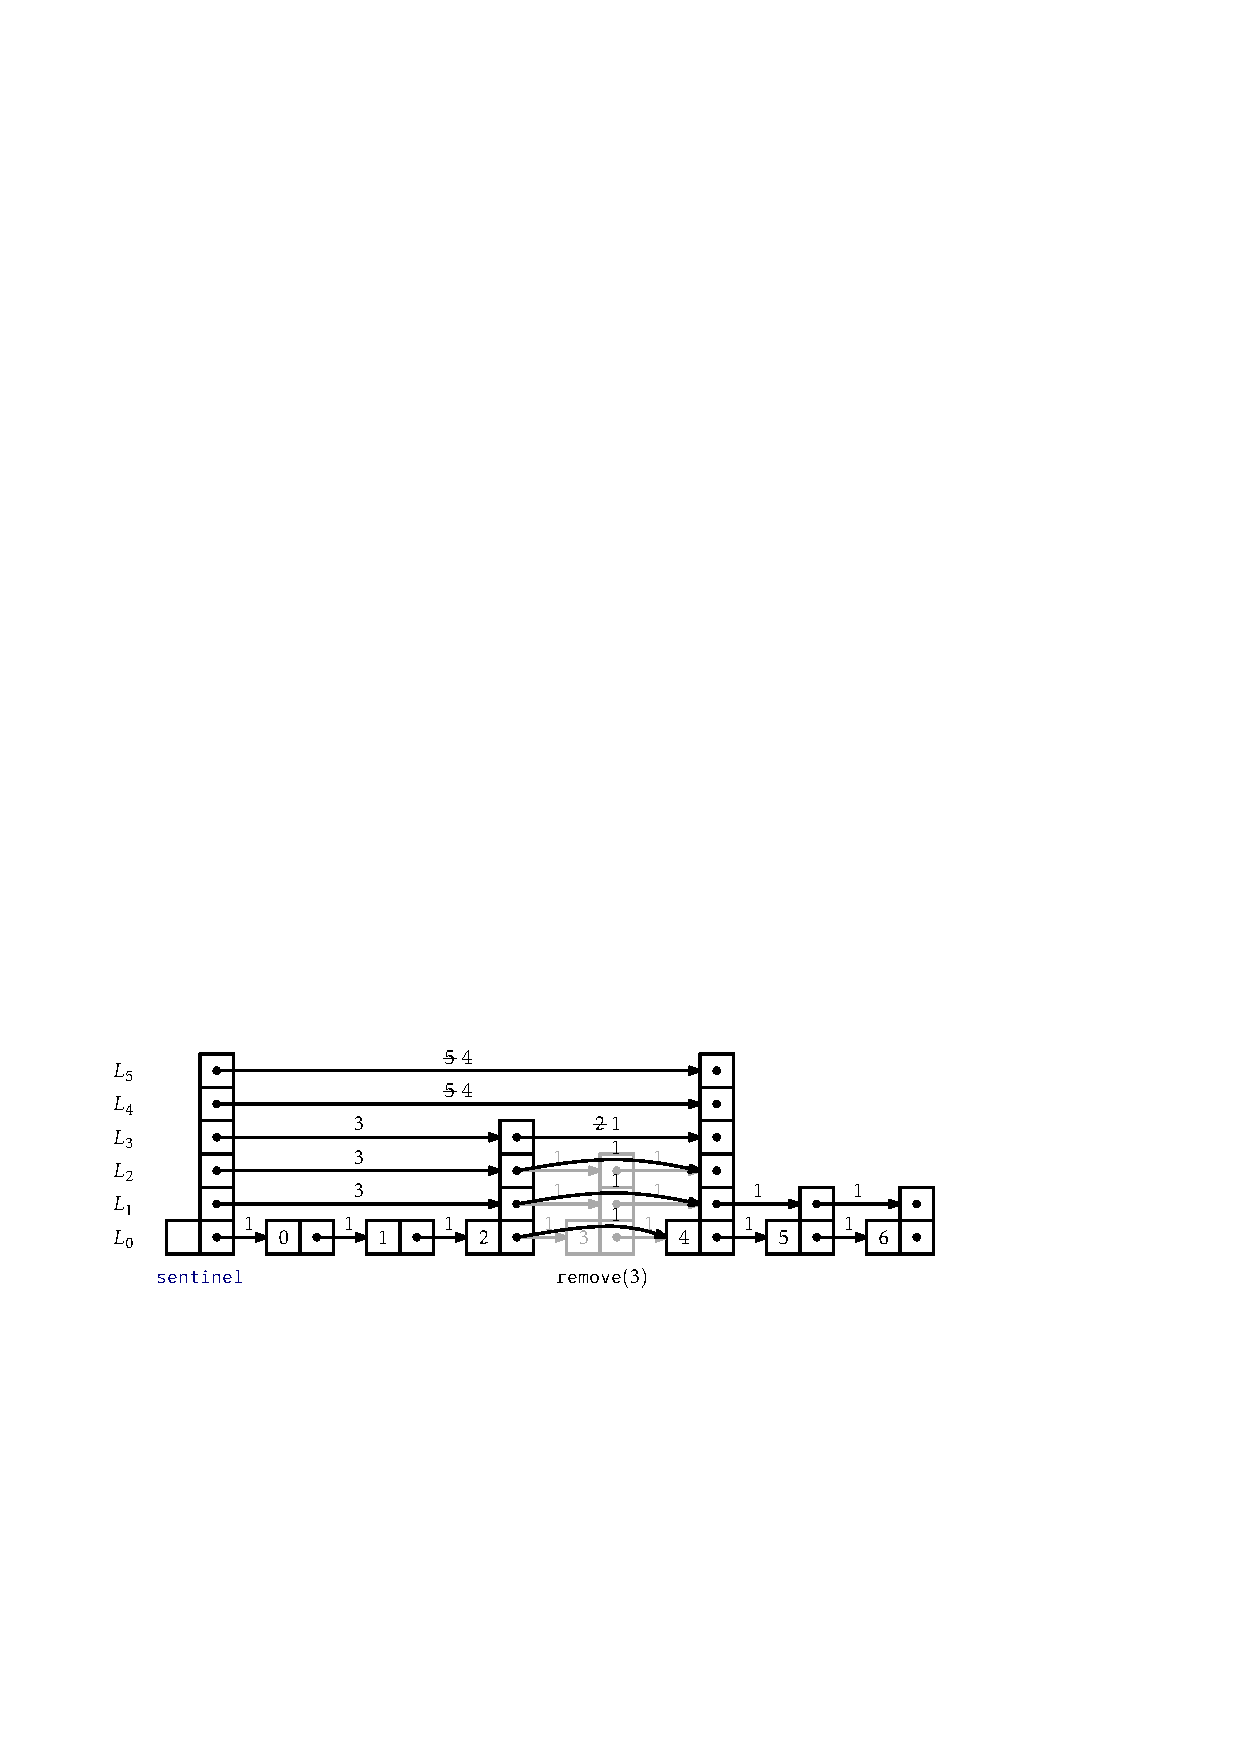
\includegraphics[width=\ScaleIfNeeded]{figs/skiplist-removei}
  \end{center}
  \caption[Removing an element from a SkiplistList]{Removing an element from a #SkiplistList#.}
  \figlabel{skiplist-removei}
\end{figure}
\codeimport{ods/SkiplistList.remove(i)}

\subsection{Summary}

The following theorem summarizes the performance of the #SkiplistList#
data structure:

\begin{thm}\thmlabel{skiplistlist}
  A #SkiplistList# implements the #List# interface.  A #SkiplistList#
  supports the operations #get(i)#, #set(i,x)#, #add(i,x)#, and
  #remove(i)# in $O(\log #n#)$ expected time per operation.
\end{thm}

%\section{Skiplists as Ropes}
%TODO: A section on ropes

\section{Analysis of Skiplists}
\seclabel{skiplist-analysis}

In this section, we analyze the expected height, size, and length of
the search path in a skiplist.  This section requires a background in
basic probability.  Several proofs are based on the following basic
observation about coin tosses.
%fim Gabriel

%inicio Lucas
\begin{lem}\lemlabel{coin-tosses}
  \index{coin toss}%
  Let $T$ be the number of times a fair coin is tossed up to and including
  the first time the coin comes up heads.  Then $\E[T]=2$.
\end{lem}

\begin{proof}
  Suppose we stop tossing the coin the first time it comes up
  heads. Define the indicator variable
  \[ I_{i} = \left\{\begin{array}{ll}
     0 & \mbox{if the coin is tossed less than $i$ times} \\
     1 & \mbox{if the coin is tossed $i$ or more times} 
     \end{array}\right.
  \]
  Note that $I_i=1$ if and only if the first $i-1$ coin tosses are tails,
  so $\E[I_i]=\Pr\{I_i=1\}=1/2^{i-1}$.  Observe that $T$, the total
  number of coin tosses, can be written as $T=\sum_{i=1}^{\infty} I_i$.
  Therefore,
  \begin{align*}
    \E[T] & =  \E\left[\sum_{i=1}^\infty I_i\right] \\
     & =  \sum_{i=1}^\infty \E\left[I_i\right] \\
     & =  \sum_{i=1}^\infty 1/2^{i-1} \\
     & =  1 + 1/2 + 1/4 + 1/8 + \cdots \\
     & =  2 \enspace .   \qedhere
  \end{align*} 
\end{proof}

The next two lemmata tell us that skiplists have linear size:

\begin{lem}\lemlabel{skiplist-size1}
  The expected number of nodes in a skiplist containing $#n#$ elements,
  not including occurrences of the sentinel, is $2#n#$.
\end{lem}

\begin{proof}
  The probability that any particular element, #x#, is included in list
  $L_{#r#}$ is $1/2^{#r#}$, so the expected number of nodes in $L_{#r#}$
  is $#n#/2^{#r#}$.\footnote{See \secref{randomization} to see how this
  is derived using indicator variables and linearity of expectation.}
  Therefore, the total expected number of nodes in all lists is
  \[ \sum_{#r#=0}^\infty #n#/2^{#r#} = #n#(1+1/2+1/4+1/8+\cdots) = 2#n# \enspace . \qedhere \]
\end{proof}

\begin{lem}\lemlabel{skiplist-height}
  The expected height of a skiplist containing #n# elements is at most
  $\log #n# + 2$.
\end{lem}

\begin{proof}
  For each $#r#\in\{1,2,3,\ldots,\infty\}$, 
  define the indicator random variable
  \[ I_{#r#} = \left\{\begin{array}{ll}
     0 & \mbox{if $L_{#r#}$ is empty} \\
     1 & \mbox{if $L_{#r#}$ is non-empty}
     \end{array}\right.
  \]
  The height, #h#, of the skiplist is then given by
  \[
       #h# = \sum_{r=1}^\infty I_{#r#} \enspace .
  \]
  Note that $I_{#r#}$ is never more than the length, $|L_{#r#}|$, of $L_{#r#}$, so 
  \[
     \E[I_{#r#}] \le \E[|L_{#r#}|] = #n#/2^{#r#} \enspace .
  \]
  Therefore, we have
  \begin{align*}
       \E[#h#] &= \E\left[\sum_{r=1}^\infty I_{#r#}\right] \\
        &= \sum_{#r#=1}^{\infty} E[I_{#r#}] \\
        &= \sum_{#r#=1}^{\lfloor\log #n#\rfloor} E[I_{#r#}]
                 + \sum_{r=\lfloor\log #n#\rfloor+1}^{\infty} E[I_{#r#}]  \\
        &\le \sum_{#r#=1}^{\lfloor\log #n#\rfloor} 1
                 + \sum_{r=\lfloor\log #n#\rfloor+1}^{\infty} #n#/2^{#r#} \\
        &\le \log #n#
                 + \sum_{#r#=0}^\infty 1/2^{#r#} \\
        &= \log #n# + 2 \enspace . \qedhere
  \end{align*}
\end{proof}

\begin{lem}\lemlabel{skiplist-size2}
  The expected number of nodes in a skiplist containing $#n#$ elements,
  including all occurrences of the sentinel, is $2#n#+O(\log #n#)$.
\end{lem}
%fim Lucas

%inicio Matheus
\begin{proof}
  By \lemref{skiplist-size1}, the expected number of nodes, not
  including the sentinel, is $2#n#$.  The number of occurrences of
  the sentinel is equal to the height, $#h#$, of the skiplist so, by
  \lemref{skiplist-height} the expected number of occurrences of the
  sentinel is at most $\log #n#+2 = O(\log #n#)$.
\end{proof}



\begin{lem}
The expected length of a search path in a skiplist is at most $2\log #n# + O(1)$.
\end{lem}

\begin{proof}
  The easiest way to see this is to consider the \emph{reverse search
  path} for a node, #x#.  This path starts at the predecessor of #x#
  in $L_0$.  At any point in time, if the path can go up a level, then
  it does.  If it cannot go up a level then it goes left.  Thinking about
  this for a few moments will convince us that the reverse search path for
  #x# is identical to the search path for #x#, except that it is reversed.

  The number of nodes that the reverse search path visits at a particular
  level, #r#, is related to the following experiment:  Toss a coin.
  If the coin comes up as heads, then move up and stop. Otherwise, move
  left and repeat the experiment.  The number of coin tosses before
  the heads represents the number of steps to the left that a reverse
  search path takes at a particular level.\footnote{Note that this
  might overcount the number of steps to the left, since the experiment
  should end either at the first heads or when the search path reaches
  the sentinel, whichever comes first. This is not a problem since the
  lemma is only stating an upper bound.} \lemref{coin-tosses} tells us
  that the expected number of coin tosses before the first heads is 1.

  Let $S_{#r#}$ denote the number of steps the forward search path takes at level
  $#r#$ that go to the right.   We have just argued that $\E[S_{#r#}]\le
  1$.  Furthermore, $S_{#r#}\le |L_{#r#}|$, since we can't take more steps
  in $L_{#r#}$ than the length of $L_{#r#}$, so
  \[
    \E[S_{#r#}] \le \E[|L_{#r#}|] = #n#/2^{#r#} \enspace .
  \]
  We can now finish as in the proof of \lemref{skiplist-height}.
  Let $S$ be  the length of the search path for some node, #u#, in a
  skiplist, and let $#h#$ be the height of the skiplist.  Then
  \begin{align*}
      \E[S] 
         &= \E\left[ #h# + \sum_{#r#=0}^\infty S_{#r#} \right] \\
         &= \E[#h#] + \sum_{#r#=0}^\infty \E[S_{#r#}]  \\
         &= \E[#h#] + \sum_{#r#=0}^{\lfloor\log #n#\rfloor} \E[S_{#r#}] 
              + \sum_{#r#=\lfloor\log #n#\rfloor+1}^\infty \E[S_{#r#}] \\
         &\le \E[#h#] + \sum_{#r#=0}^{\lfloor\log #n#\rfloor} 1
              + \sum_{r=\lfloor\log #n#\rfloor+1}^\infty #n#/2^{#r#} \\
         &\le \E[#h#] + \sum_{#r#=0}^{\lfloor\log #n#\rfloor} 1
              + \sum_{#r#=0}^{\infty} 1/2^{#r#} \\
         &\le \E[#h#] + \sum_{#r#=0}^{\lfloor\log #n#\rfloor} 1
              + \sum_{#r#=0}^{\infty} 1/2^{#r#} \\
         &\le \E[#h#] + \log #n# + 3 \\
         &\le 2\log #n# + 5  \enspace . \qedhere
  \end{align*}
\end{proof}


The following theorem summarizes the results in this section:
\begin{thm}
A skiplist containing $#n#$ elements has expected size $O(#n#)$ and the
expected length of the search path for any particular element is at most
$2\log #n# + O(1)$.
\end{thm}



%\section{Iteration and Finger Search}

%TODO: Write this section

\section{Discussion and Exercises}

Skiplists were introduced by Pugh \cite{p91} who also presented
a number of applications and extensions of skiplists \cite{p89}.  Since then they
have been studied extensively.  Several researchers have done very
precise analyses of the expected length and variance of the length of the
search path for the #i#th element in a skiplist \cite{kp94,kmp95,pmp92}.
Deterministic versions \cite{mps92}, biased versions \cite{bbg02,esss01},
and self-adjusting versions \cite{bdl08} of skiplists have all been
developed.  Skiplist implementations have been written for various
languages and frameworks and have been used in open-source database
systems \cite{skipdb,redis}. A variant of skiplists is used in the HP-UX
operating system kernel's process management structures \cite{hpux}.
\javaonly{Skiplists are even part of the Java 1.6 API \cite{oracle_jdk6}.}
%fim Matheus

%inicio Pedro

\begin{exc}
  Illustrate the search paths for 2.5 and 5.5 on the skiplist in 
  \figref{skiplist}.
\end{exc}

\begin{exc}
  Illustrate the addition of the values 0.5 (with a height of 1) and
  then 3.5 (with a height of 2) to the skiplist in \figref{skiplist}.
\end{exc}

\begin{exc}
  Illustrate the removal of the values 1 and then 3  from the skiplist
  in \figref{skiplist}.
\end{exc}

\begin{exc}
  Illustrate the execution of #remove(2)# on the #SkiplistList#
  in \figref{skiplist-lengths}.
\end{exc}

\begin{exc}
  Illustrate the execution of #add(3,x)# on the #SkiplistList#
  in \figref{skiplist-lengths}.  Assume that #pickHeight()# selects a height
  of 4 for the newly created node.
\end{exc}

\begin{exc}\exclabel{skiplist-changes}
  Show that, during an #add(x)# or a #remove(x)# operation, the expected
  number of pointers in a #SkiplistSet# that get changed is constant.
\end{exc}

\begin{exc}\exclabel{skiplist-opt}
  Suppose that, instead of promoting an element from $L_{i-1}$ into $L_i$
  based on a coin toss, we promote it with some probability $p$, $0 <
  p < 1$.
  \begin{enumerate}
   \item Show that, with this modification, the expected length of a
     search path is at most $(1/p)\log_{1/p} #n# + O(1)$.
   \item What is the value of $p$ that minimizes the preceding expression?
   \item What is the expected height of the skiplist? 
   \item What is the expected number of nodes in the skiplist?
  \end{enumerate}
\end{exc}


\begin{exc}\exclabel{skiplist-opt-2}
  The #find(x)# method in a #SkiplistSet# sometimes performs
  \emph{redundant comparisons}; these occur when #x# is compared to the
  same value more than once.  They can occur when, for some node, #u#,
  $#u.next[r]# = #u.next[r-1]#$.  Show how these redundant comparisons
  happen and modify #find(x)# so that they are avoided.  Analyze the
  expected number of comparisons done by your modified #find(x)# method.
\end{exc}

\begin{exc}
  Design and implement a version of a skiplist that implements the
  #SSet# interface, but also allows fast access to elements by rank.
  That is, it also supports the function #get(i)#, which returns the
  element whose rank is #i# in $O(\log #n#)$ expected time. (The rank
  of an element #x# in an #SSet# is the number of elements in the #SSet#
  that are less than #x#.)
\end{exc}

\begin{exc}
  \index{finger}%
  \index{finger search!in a skiplist}%
  A \emph{finger} in a skiplist is an array that stores the
  sequence of nodes on a search path at which the search path
  goes down. (The variable #stack# in the #add(x)# code on
  page~\pageref{pg:skiplist-add} is a finger;  the shaded nodes in
  \figref{skiplist-add} show the contents of the finger.)  One can
  think of a finger as pointing out the path to a node in the lowest
  list, $L_0$.

  A \emph{finger search} implements the #find(x)# operation using a
  finger, by walking up the list using the finger until reaching a node
  #u# such that $#u.x# < #x#$ and $#u.next#=#null#$ or $#u.next.x# >
  #x#$ and then performing a normal search for #x# starting from #u#.
  It is possible to prove that the expected number of steps required
  for a finger search is $O(1+\log r)$, where $r$ is the number values
  in $L_0$ between #x# and the value pointed to by the finger.
%fim Matheus

%inicio Rodrigo
  Implement a subclass of #Skiplist# called #SkiplistWithFinger# that
  implements #find(x)# operations using an internal finger.  This subclass
  stores a finger, which is then used so that every #find(x)# operation
  is implemented as a finger search.  During each #find(x)# operation
  the finger is updated so that each #find(x)# operation uses, as a
  starting point, a finger that points to the result of the previous
  #find(x)# operation.
\end{exc}

\begin{exc}\exclabel{skiplist-truncate}
  Write a method, #truncate(i)#, that truncates a #SkiplistList#
  at position #i#.  After the execution of this method, the size
  of the list is #i# and it contains only the elements at indices
  $0,\ldots,#i#-1$.  The return value is another #SkiplistList# that
  contains the elements at indices $#i#,\ldots,#n#-1$.  This method
  should run in $O(\log #n#)$ time.
\end{exc}

\begin{exc}
  Write a #SkiplistList# method, #absorb(l2)#, that takes as an
  argument a #SkiplistList#, #l2#, empties it and appends its contents,
  in order, to the receiver.  For example, if #l1# contains $a,b,c$
  and #l2# contains $d,e,f$, then after calling #l1.absorb(l2)#, #l1#
  will contain $a,b,c,d,e,f$ and #l2# will be empty. This method should
  run in $O(\log #n#)$ time.
\end{exc}

\begin{exc}
  Using the ideas from the space-efficient list, #SEList#, design
  and implement a space-efficient #SSet#, #SESSet#.  To do this, store the
  data, in order, in an #SEList#, and store the blocks of this #SEList#
  in an #SSet#. If the original #SSet# implementation uses $O(#n#)$
  space to store #n# elements, then the #SESSet# will use enough space
  for #n# elements plus $O(#n#/#b#+#b#)$ wasted space.
\end{exc}

\begin{exc}
  Using an #SSet# as your underlying structure, design and implement an
  application that reads a (large) text file and allows you to search,
  interactively, for any substring contained in the text.  As the user
  types their query, a matching part of the text (if any) should appear 
  as a result.

  \noindent  Hint 1: Every substring is a prefix of some suffix, so it
  suffices to store all suffixes of the text file.

  \noindent Hint 2:  Any suffix can be represented compactly as a single
  integer indicating where the suffix begins in the text.

  \noindent Test your application on some large texts, such as some of
  the books available at Project Gutenberg \cite{gutenberg}.  If done
  correctly, your applications will be very responsive; there should be
  no noticeable lag between typing keystrokes and seeing the results.
\end{exc}

\begin{exc}
  \index{skiplist!versus binary search tree}%
  \index{binary search tree!versus skiplist}%
  (This exercise should be done after reading about binary search trees,
  in \secref{binarysearchtree}.)  Compare skiplists with binary search
  trees in the following ways:  
  \begin{enumerate}
     \item Explain how removing some edges of a skiplist leads to
       a structure that looks like a binary tree and is similar to a
       binary search tree.
     \item Skiplists and binary search trees each use about the same
       number of pointers (2 per node).  Skiplists make better use of
       those pointers, though. Explain why.
  \end{enumerate}
\end{exc}
%fim Rodrigo